\documentclass[12pt]{article}
\linespread{1.15}

\usepackage[top=1.5cm, right=2cm, left=2cm]{geometry}
\usepackage{graphicx}
\usepackage[section]{placeins}
\usepackage[hidelinks, urlcolor=blue]{hyperref}
\usepackage{float}
\usepackage[perpage, stable]{footmisc}
\usepackage{amsmath}
\usepackage{titling}
\usepackage{tabularx}
\usepackage{booktabs}


% Commands
\newcommand{\column}[1]{\textit{#1}}

\newcommand{\fm}{Fashion MNIST}
\newcommand{\pca}{PCA}
\renewcommand{\ae}{Autoencoder}

% Custom title page setup
\makeatletter
\def\maketitle{
	\begin{titlepage}
		\begin{center}
			\vspace*{2cm}
			
			{\Large\bfseries Machine Learning Course\par}
			\vspace{2cm}
			
			{\Huge\bfseries Noise Reduction Using PCA and Autoencoder Assignment Report\par}
			\vspace{3cm}
			
			{\large\bfseries Professor:\par}
			{\large Dr. Mahdi Eftekhari\par}
			\vspace{1.5cm}
			
			{\large\bfseries Author:\par}
			{\large Amirhossein Abolhassani\par}
			\vspace{2cm}
			
			\vfill  % pushes the date to bottom
			
			{\large\bfseries Fall 2024}
			
		\end{center}
	\end{titlepage}
	\setcounter{page}{1}
}
\makeatother

\begin{document}
	\maketitle
	\tableofcontents
	\newpage
	\section{Introduction}
	One of the tasks in image processing is Noise Reduction. This task aims to reduce image noise using various algorithms and techniques. Two fundamental techniques are explored in this assignment and tested on the Fashion MNIST dataset:
	\begin{itemize}
		\item Principal Component Analysis (PCA)
		\item Autoencoder
	\end{itemize}
	\section{Dataset Description}
	The Fashion MNIST dataset is widely used in machine learning and computer vision. It consists of grayscale images of various clothing and accessories, serving as a modern alternative to the classic MNIST dataset. A sample of the data is shown in Figure \ref{fig: fmn data}.
	\begin{figure}[H]
		\centering
		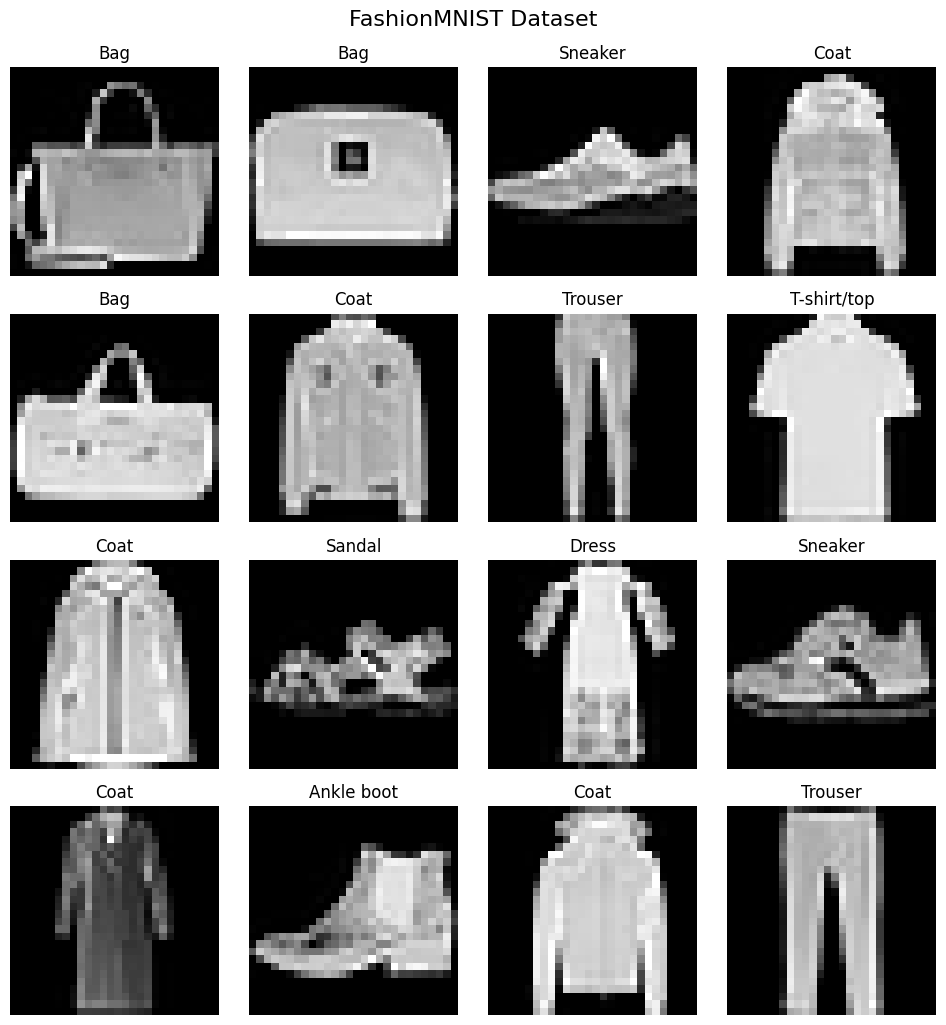
\includegraphics[scale=0.45]{figs/fmn data raw}
		\caption{Subset of the \fm dataset}
		\label{fig: fmn data}
	\end{figure}
	\begin{table}[H]
		\centering
		\begin{tabularx}{\linewidth}{|X|X|}
			\toprule
			Total number of images & 70,000 \\
			\midrule
			Training set & 60,000 \\
			\midrule
			Test set & 10,000 \\
			\midrule
			Image dimensions & 28×28 pixels \\
			\midrule
			Image type & Grayscale (single-channel) \\
			\midrule
			Pixel value range & 0 to 255 \\
			\bottomrule
		\end{tabularx}
		\caption{Characteristics of the Fashion MNIST dataset}
		\label{tbl: fMNIST Chars}
	\end{table}
	The dataset includes 10 distinct classes:
	\begin{itemize}
		\item T-shirt/top
		\item Trousers
		\item Pullover
		\item Dress
		\item Coat
		\item Sandal
		\item Shirt
		\item Sneaker
		\item Bag
		\item Ankle boot
	\end{itemize}	
	\section{Adding Gaussian Noise to the Dataset}
	Gaussian Noise is a type of noise added to images. The following probability density function describes this noise in two dimensions, as applied to images:
	\[ n(x,y) = \frac{1}{2\pi\sigma^2} e^{-\frac{(x-\mu_x)^2 + (y-\mu_y)^2}{2\sigma^2}} \]
		\begin{tabular}{l | l}
			$\mu$ & Mean \\
			$\sigma$ & Standard deviation, indicating noise spread \\
			$\sigma^2$ & Variance \\
		\end{tabular}
	\newpage
	\noindent
	In image processing, the formula for adding Gaussian noise to an image is:
	\[
	g(x,y) = f(x,y) + n(x,y)
	\]
	
		\begin{tabular}{l | l}
			$g(x,y)$ & Noisy image \\
			$f(x,y)$ & Original image \\
			$n(x,y)$ & Gaussian noise following a normal distribution with specified mean and standard deviation \\
		\end{tabular}\\
	
	Initially, Gaussian noise with a variance of 1.0 and mean of 0 is added to the \fm dataset. These noisy images are used throughout the assignment.\footnote{In practice, each image is converted to a vector of length 784 for use in this assignment.} (A subset of the noisy dataset is shown in Figure \ref{fig: fmn data noisy}.)
	\begin{figure}[H]
		\centering
		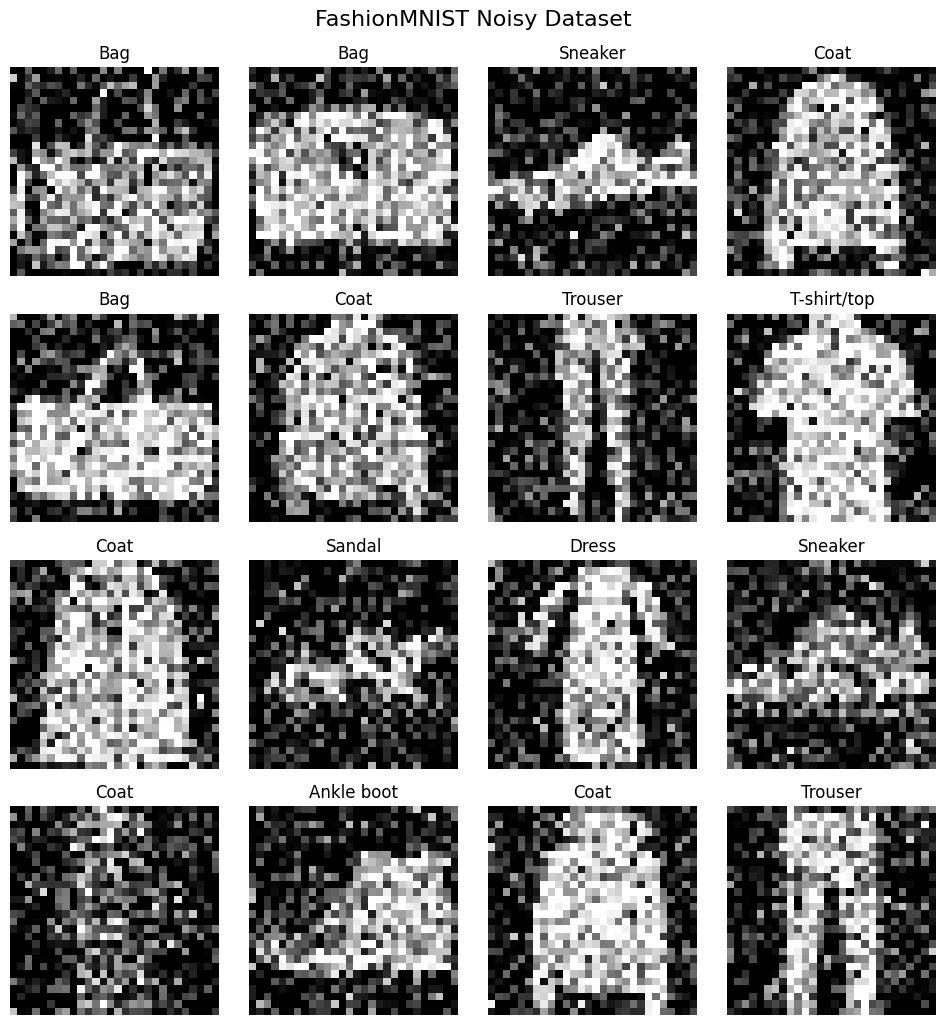
\includegraphics[scale=0.5]{figs/fmn data noisy}
		\caption{Subset of the noisy \fm dataset}
		\label{fig: fmn data noisy}
	\end{figure}
	\newpage
	\section{Noise Reduction with \pca}\label{sec: pca}
	PCA, as a linear dimensionality reduction method, preserves important data components. By treating noise as less significant information, PCA is expected to reduce noise in images. The process involves computing the matrix \( Q \)\footnote{The matrix \( Q \) contains orthogonal unit vectors, so \( Q^{-1} = Q^T \).}, which includes the eigenvectors of the covariance matrix \( \Sigma \):
	\[
	\Sigma = Q\Lambda Q^{-1}
	\]
	\[
	Q = [q_1 \; q_2 \; \cdots \; q_d]
	\]
	\[
	\lambda_1 \geq \lambda_2 \geq \cdots \geq \lambda_d
	\]
	Then, the data is projected onto the principal components:
	\[
	Y = (X - \mu)Q
	\]
	Finally, the data is reconstructed to its original dimensionality:
	\[
	X' = YQ^T + \mu
	\]
	By selecting an appropriate number of principal components, this dimensionality reduction and reconstruction process is expected to remove significant noise from the image.\\
	In this assignment, 80 principal components yielded the best result among 784 possible components, achieving a reconstruction error of 0.0239, the lowest among tested values (Figure \ref{fig: pca best k}).
	\begin{figure}[H]
		\centering
		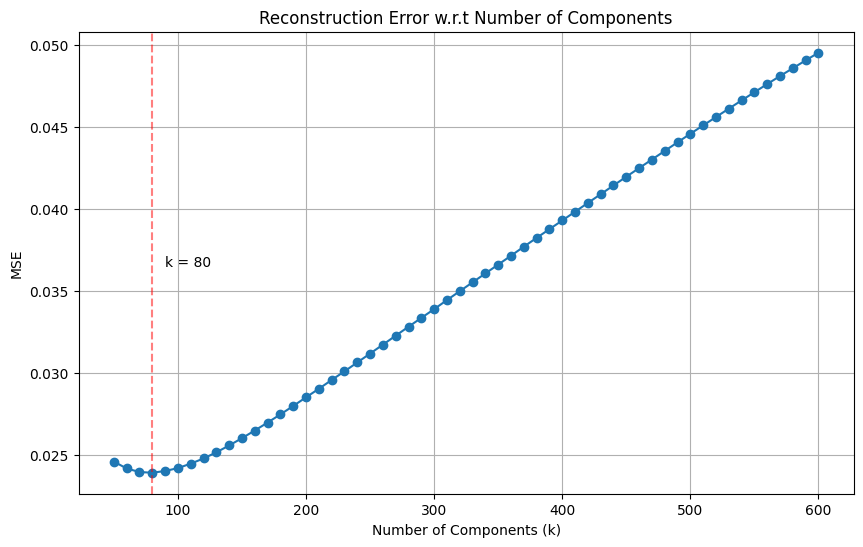
\includegraphics[scale=0.6]{figs/best k pca}
		\caption{Finding the optimal number of components based on reconstruction error}
		\label{fig: pca best k}
	\end{figure}
	\section{Noise Reduction with \ae}\label{sec: ae}
	An Autoencoder is a neural network consisting of an Encoder and a Decoder. It can perform linear (with linear activation functions) or nonlinear (with nonlinear activation functions) dimensionality reduction.\\
	One application of this architecture is to input noisy images and use the corresponding clean images as labels, training the Autoencoder to map noisy images to clean ones, which is the desired model.\\
	A PyTorch-based network with Dense layers and ReLU activation functions was implemented. The layer structure is as follows:
	\[
	\text{Encoder}: 784 \rightarrow 512 \rightarrow 256 \rightarrow 128
	\]
	\[
	\text{Decoder}: 128 \rightarrow 256 \rightarrow 512 \rightarrow 784
	\]
	Figure \ref{fig: ae train test error} shows the training and test error trends, indicating proper learning without overfitting. With the hyperparameters listed in Table \ref{tbl: ae hyparam}, an error of 0.013 was achieved.
	\begin{figure}[H]
		\centering
		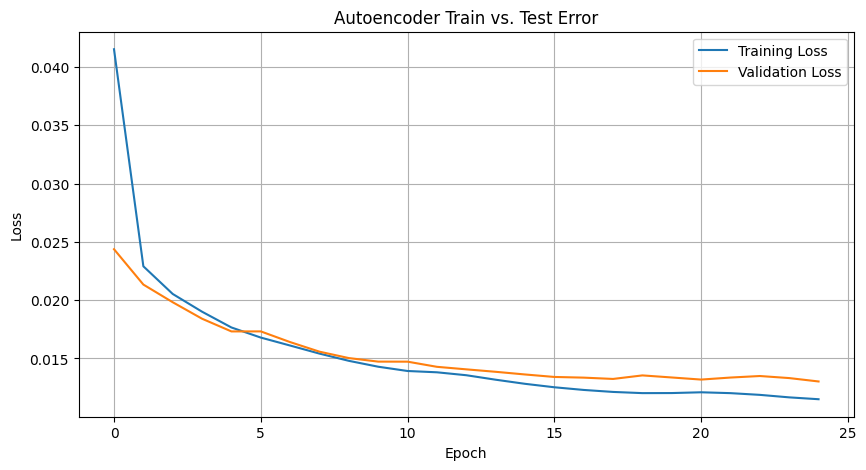
\includegraphics[scale=0.6]{figs/train test error ae}
		\caption{Training and test error trends for the Autoencoder}
		\label{fig: ae train test error}
	\end{figure}
	\begin{table}[H]
		\centering
		\begin{tabularx}{\linewidth}{|X|X|}
			\toprule
			Learning rate & 0.001 \\
			\midrule
			Batch size & 128 \\
			\midrule
			Epochs & 25 \\
			\bottomrule
		\end{tabularx}
		\caption{Hyperparameters for the Autoencoder}
		\label{tbl: ae hyparam}
	\end{table}
	\section{Results}\label{sec: results}
	Comparing the errors reported in Sections \ref{sec: ae} and \ref{sec: pca}, the Autoencoder is expected to outperform PCA in noise reduction. Figure \ref{fig: method comparison} compares the noisy image, original image, PCA-denoised image, and Autoencoder-denoised image.
	\begin{figure}[H]
		\centering
		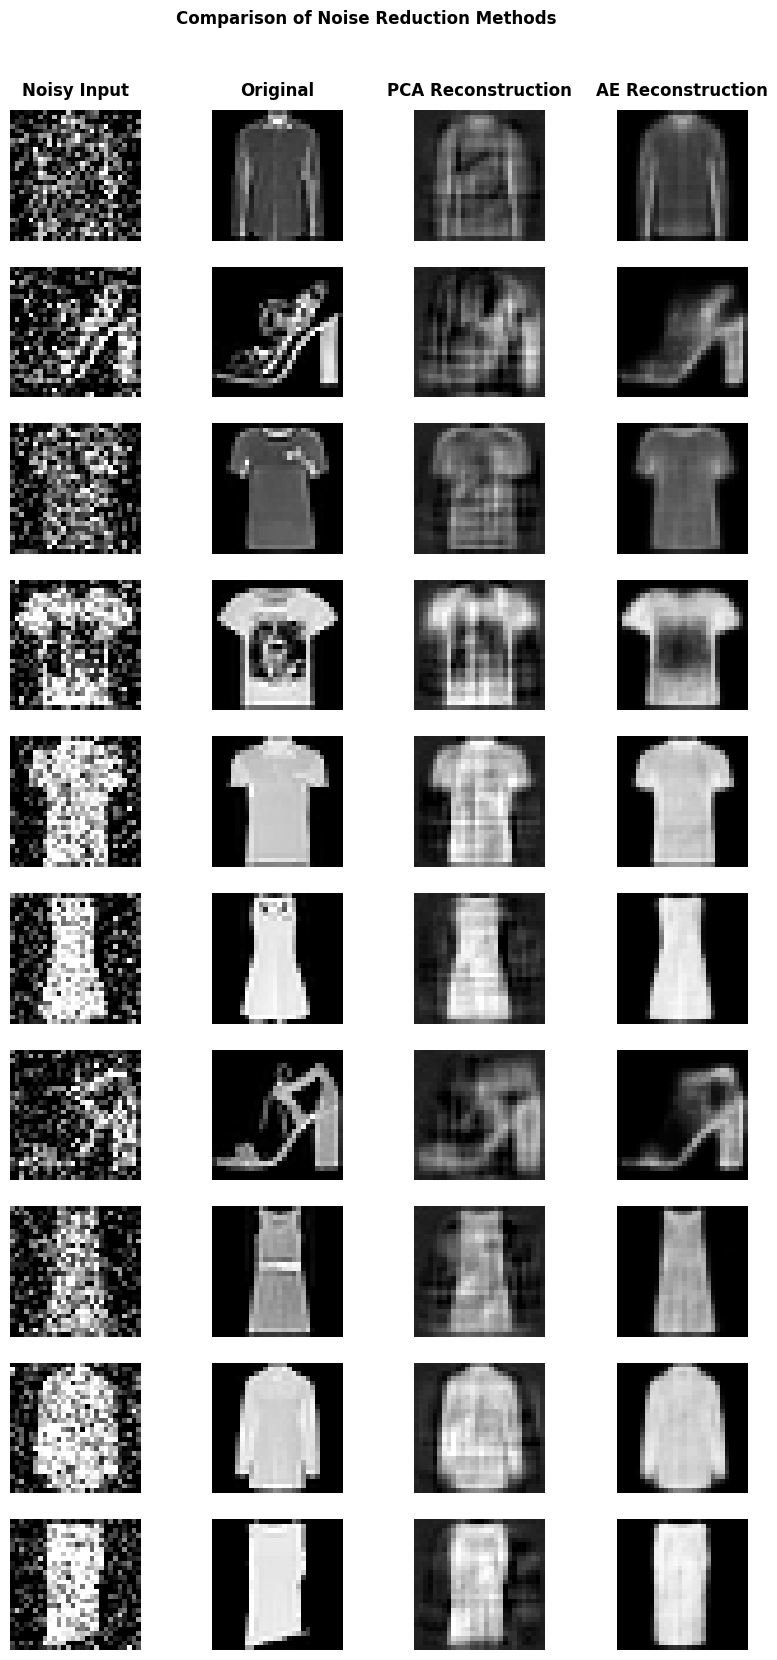
\includegraphics[scale=0.45]{figs/resutl comparison}
		\caption{Comparison of noise reduction results}
		\label{fig: method comparison}
	\end{figure}
	\section{A Challenge: Fair Comparison}
	The biggest challenge in this assignment was ensuring a fair comparison. The dataset was downloaded once, and noise was added only once to ensure consistency across methods. This was critical because Scikit Learn was used for PCA, and PyTorch was used for the Autoencoder. Adding noise separately for each method could lead to inconsistencies, and loading the dataset separately for each method would cause redundancy. Thus, the dataset was downloaded and noised once, used consistently throughout, ensuring a fair comparison.
	
	\section{Conclusion}
	Based on the results in Section \ref{sec: results}, both methods effectively reduced noise, but the Autoencoder outperformed PCA. This is likely due to the Autoencoder’s ability to capture nonlinear relationships, unlike PCA, which is limited to linear relationships.
	
\end{document}